\section{September 2023: LibrePCB 1.0.0}

\begin{frame}{\secname}
  \begin{itemize}
    \item<1-> Advanced PCB features (thermal reliefs, blind \& buried vias, slotted pads, \ldots)
    \item<2-> 3D PCB viewer \& STEP export
    \item<3-> Assembly variants \& MPN management
      \begin{itemize}
        \item Adding MPNs to libraries
        \item Specifying MPNs in schematics
        \item Alternate (second-source) MPNs
        \item Different parts in each assembly variant
        \item Separate BOM for each assembly variant
      \end{itemize}
    \item<4-> Output jobs
      \begin{itemize}
        \item Unified export for any kind of production data
        \item Highly customizable
        \item 100\% reproducible/portable
        \item Runnable from GUI and CLI
      \end{itemize}
  \end{itemize}

  \begin{tikzpicture}[remember picture,overlay]
    \node<1>[xshift=0cm,yshift=-0.5cm] at (current page.center){%
    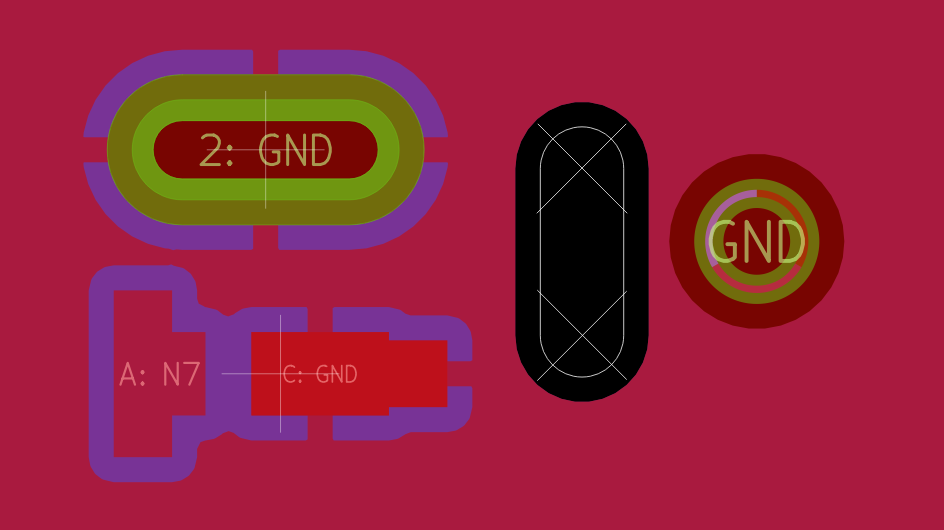
\includegraphics[height=5.5cm]{images/advanced_features.png}};

    \node<2>[xshift=0cm,yshift=-1cm] at (current page.center){%
    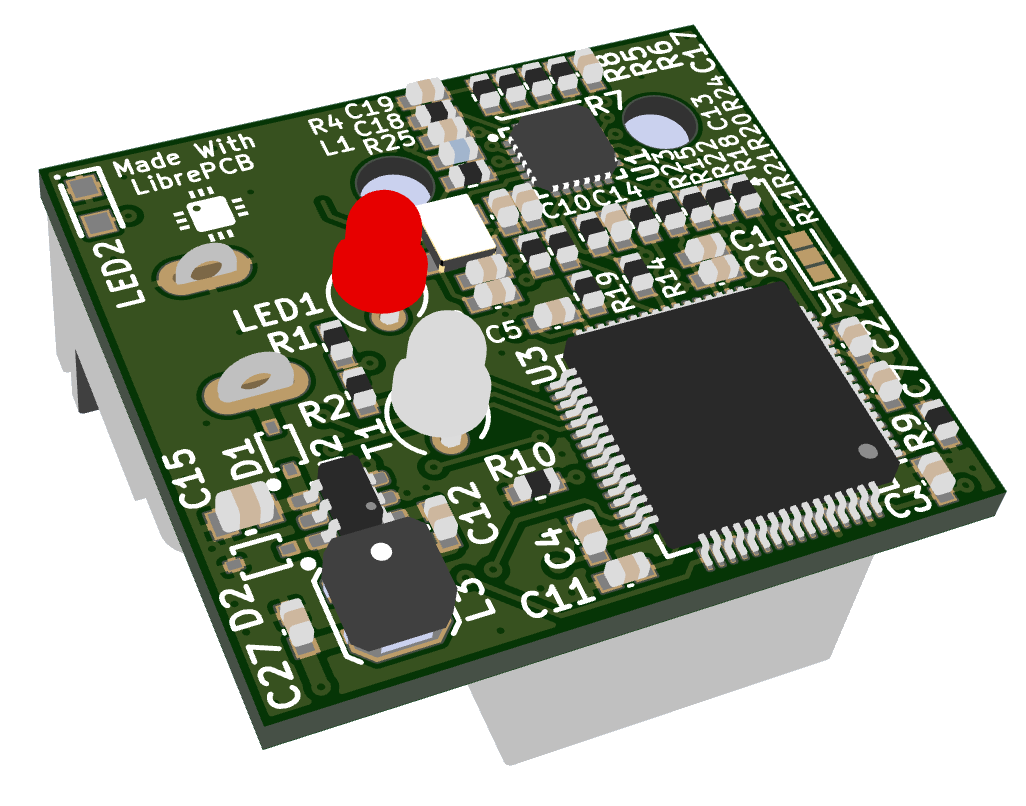
\includegraphics[width=8cm]{images/3d_viewer.png}};

    \node<3>[xshift=0cm,yshift=-2.5cm] at (current page.center){%
    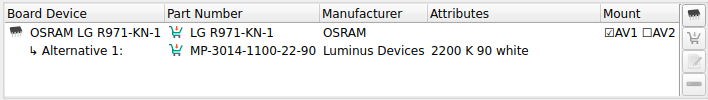
\includegraphics[width=13.5cm]{images/mpn_management.png}};

    \node<4>[xshift=4.9cm,yshift=-0.8cm] at (current page.center){%
    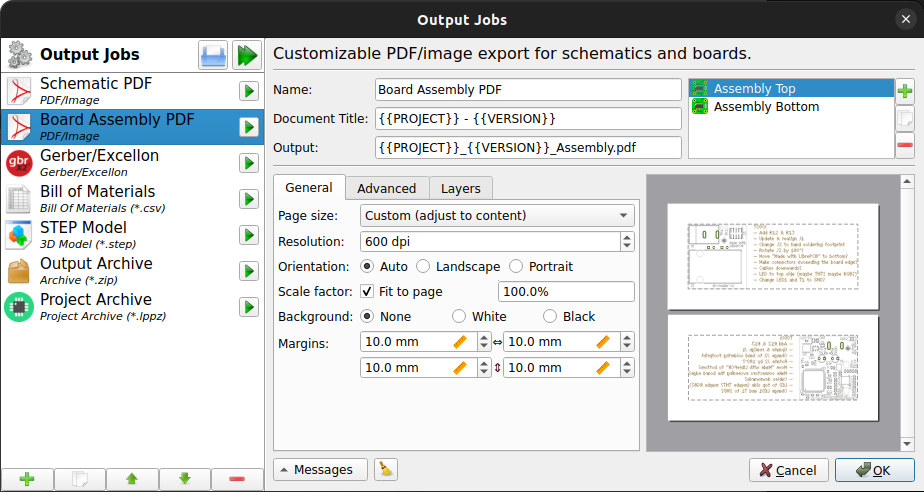
\includegraphics[trim=0 0 9.9cm 0,clip,height=5.5cm]{images/output_jobs.png}};
  \end{tikzpicture}

  \note<1>{
    But now let's take a look at the application. In September last year we
    released version 1.0 which was a very exciting moment.\\

    Beside many new capabilities of the board editor, like thermal relief pads,
  }

  \note<2>{
    this release also added a 3D board viewer with STEP model import and
    export, which is not only fancy but also a great way to review a design
    before ordering PCBs.
  }

  \note<3>{
    But I'm especially proud of two features which make generating production
    data a pleasure.\\

    First of all, we have introduced a very comprehensive support for assembly
    variants and manufacturer part number management.\\

    MPNs can now be stored in libraries so you don't need to add
    them manually to the schematic. In the schematic you can even assign
    multiple MPNs to a component to export them as second-source parts to
    the BOM. Or you can specify different parts for different assembly variants,
    for example a 10k resistor in one variant but a 0 ohm resistor in another
    variant.
  }

  \note<4>{
    And to make generating these BOMs and any other output data a matter of
    seconds, we introduced output jobs as a new, unified way to export data.\\

    These output jobs can be configured very flexible and are stored in the
    project, so the exact same output files can be reproduced on a different
    computer with just a single click.\\

    Or with the provided command-line interface you may even fully automate
    the production data generation on a continuous integration system.
  }

\end{frame}
